  %% \section*{History of Changes}
  %% \small

  %% {\bfseries 2011-11-06} Initial revision.

  %% {\bfseries 2011-11-09} Clarified behaviour of reset mechanism. Froze
  %% definition of reset signals.

  %% {\bfseries 2011-11-10} Modified Control Bus pin-out. Added description for missing bus signals.

  %% {\bfseries 2011-11-15} Modified Control Bus pin-out (revision G). Removed
  %% \OPIFn{3}–\OPIFn{0} signals. Added \IRn{2}–\IRn{0}. Corrected power
  %% pin-out. Corrected minor issue with pin-out descriptions.

  %% {\bfseries 2011-11-20} Modified Control Bus pin-out (revision H) to
  %% include \FV{} signal.

  
\section{Introduction}

The CFT design incorporates two separate buses:

\begin{description}

\item{\bfseries The Control Bus} provides a local interconnect for signals
  local to the processor part of the computer. This includes the \IBUS, signals
  from the Control Unit, and Microcode ROM, as well as signals to and from the
  \ALU, registers, interrupt controller boards, and all other processor
  units. This bus connects the three Processor Boards, but may be used for
  future processor extensions. Physically, this bus is implemented using 40×2
  pin headers, although additional pins are required for some local functions.

\item{\bfseries The Expansion Bus} is meant for 96-pin DIN 41612 ‘Bauform C’
  connectors and 100x160mm (3U) Eurocards (IEEE 1101) connected via a 19-slot
  backplane. It mainly provides a computer-level expansion interface, although
  many processor extensions can also be attached here. The Expansion Bus allows
  devices to connect to the memory space, I/O space, and expanded memory space
  by using the Address Bus, Data Bus, their associated control lines, as well
  as interrupt lines.

\end{description}

The two buses are not directly connected, but the processor boards bridge some
of their signals where and when it is appropriate.

\section{Backplane}
\label{sec:backplane}

\begin{figure}
\centering
\includeimage{figs/din41612}
\caption[A DIN41612 receptacle with power rails]{\label{fig:slot}A card
  receptacle on the CFT backplane (as seen from the top) showing the power and
  ground rails including one reserved for future expansion (which has now been
  allocated to the 3.3V rail), as well as the two local test point pins. All
  other pins are connected across the backplane and terminated at either end.
}
\end{figure}

\begin{figure}%
\centering%
\includelarge[width=0.95\columnwidth]{figs/dsc_1996b.jpg}\\
\caption[A photo of the CFT backplane.]{\label{photo:backplane}A close-up photo
  of the backplane, showing around half of its 96-pin DIN 41612 sockets, screws
  for attaching power terminals, and the pads of the termination resistors
  (located on the underside of the board). Seven bypass capacitors are visible
  along the short edge.
}
\end{figure}


The CFT backplane, shown in~\fcf{photo:backplane} is based on a part available
to the author at the time when the CFT was originally designed. Historically,
it belonged to a computer used and possibly designed at the University of
Edinburgh's Department of Computer Science. The machines were decommissioned
circa 1993 and were based on a Motorola MC68020 microprocessor.

The backplane itself is a Eurocard (IEEE 1101) design using DIN 41612
connectors. The connectors are {\em Bauform\/} (style) ‘C’ 96-pin
receptacles. A diagram of the connectors as used on this backplane may be found
in~\fcf{fig:slot}.

Five power rails are provided at the edges of the card, occupying a total of 6
rows, or 18 pins.

Of the remaining 78 pins, 2 pins per connector are not bussed. Instead, they
are broken out to test points on the backplane. This leaves 76 pins for bus
signals.

All 76 signal pins are terminated at both ends of the bus using a TTL
termination scheme. Termination resistors tie each signal to both power and
ground rails with an unbalanced pair of resistors, to aid weak TTL drivers and
to square signals, as well as to deal with transmission line problems. The
termination scheme is shown in~\fcf{fig:bus-termination}. This, of course,
forms a voltage divider:

\begin{eqnarray}
& V_{\mbox{out}} =  5\mbox{V} \frac{\displaystyle330\mbox{Ω}}{\displaystyle 330\mbox{Ω} + 470\mbox{Ω}} = 2.938\mbox{V}\nonumber
\end{eqnarray}

The termination helps weak TTL drivers source or sink current to keep waveforms
square and reduces transmission line effects. This is not an ideal termination
scheme for CMOS drivers, but the negative effects (if any) will have to be
gauged empirically.

\begin{figure*}
\centering
\includelarge[width=0.85\textwidth]{figs/bus-termination.png}\\
\caption[Backplane bus termination]{\label{fig:bus-termination}Backplane bus
  termination. Each line is terminated at each end, using a pair of resistors
  to power and ground. The 330Ω and 470Ω resistors form a voltage divider that
  produces a termination voltage of 2.9375~V on each line.}
\end{figure*}

%% Both buses share the same physical backplane. To isolate them, the
%% suggestion is to cut the traces between the last slot of the control
%% bus and the first slot of the expansion bus, and to provide
%% termination resistors on the bus bridge card.

%% If building the machine from scratch, two separate backplanes or DIN
%% 41612 connectors on ribbon cables may be used, or the constructor may
%% develop a custom {\em ad hoc\/} solution. In the interest of allowing
%% implementations on other, possibly unterminated backplanes, optional
%% bus termination will also be provided on two cards, one on the control
%% side and one on the expansion side.

\subsection{Backplane Heat Dissipation}

The backplane's termination scheme essentially makes the device an effective
5~Ω resistor. This is easy to calculate, given there are two sets of
terminating resistors for each of the 76 signals, each tied from power to
ground, each 330~Ω and 470~Ω respectively. This gives $330\mbox{Ω}+470\mbox{Ω}
= 800\mbox{Ω}$ from power to ground, per signal per terminator bank. With $2×76
= 152$ of these in parallel, the resistance is expected to be:

\begin{eqnarray}
R_{\mbox{\em backplane}} &=& \frac{1}{152×(800\mbox{Ω})^{-1}} = \nonumber\\
                  &=& 5.263\mbox{Ω}\nonumber
\end{eqnarray}

\noindent At 5~V, by Ohm's Law, the current through the backplane is

\begin{eqnarray}
I_{\mbox{\em backplane}} &=& \frac{5\mbox{V}}{5.263\mbox{Ω}} = 0.95\mbox{A}\nonumber
\end{eqnarray}

This is equivalent to $0.95\mbox{A}×5\mbox{V} = 4.75\mbox{W}$ of power, or
approximately $4.75\mbox{W} ÷ 14 = 340\mbox{mW}$ of power per 16-pin \gls{DIP}
resistor net. This is converted to heat, which should be removed from the
surface of the resistor nets with a heatsink and/or fan, otherwise the
temperature will change the resistance and thus the characteristics of the
circuit.

\section{Control Bus}

\todo{Being revised!}

The Control Bus provides an interconnect for signals local to the processor
part of the computer. Anything peripherals don't need to use (or shouldn't be
using!) is on the Control Bus. This includes the \IBUS, signals from the
Control Unit and Microcode ROM, as well as signals to and from the \ALU,
register boards, interrupt controller boards, and all other processor
components.

The Control Bus is implemented as a pair of 2×20-pin 2.54mm headers, identical
to the ones used for parallel IDE devices. This makes it cheaper to source
cable and plugs, since most people likely to be reading this will have mmore
parallel IDE cables lying around than they know what to do with. Two
40-conductor flat cables connect all the cards using the control bus in a
daisy-chain fashion. The two pin headers are referred to as P1 and P2, with
pins designated P1.1–P1.40 and P2.1–P2.40.

Even though this is a processor-local bus, trace length is probably long enough
for transmission line effects, so all output signals are conditioned using
either impedance-matching resistors in series or bus hold circuitry.

There are six signals that normally belong to the Control Bus, but have been
relegated to the Expansion Bus because of lack of available pins. These are
signals that expansion boards (however exotic) could potentially benefit from.

\begin{table}[t]
\caption{\label{table-control-pinout}Control Bus Pin-out.}
\vspace{1em}
\centering
\zebra
\begin{tabular}{*{4}{rp{0.14\columnwidth}}}
%\noalign{\smallskip}\hline\noalign{\smallskip}
%\\\hline
Pin & Signal & Pin & Signal & Pin & Signal & Pin & Signal \\
%\noalign{\smallskip}\hline\noalign{\smallskip}
\hline
P1.1  & \CLL        & P1.2  & \CPL       & P2.1  & \STPAC     & P2.2  & \STPDR     \\
P1.3  & \ns{RAGL}   & P1.4  & \ns{WALU}  & P2.3  & \INCPC     & P2.4  & \RAC       \\
P1.5  & \FL         & P1.6  & \FV        & P2.5  & \RDR       & P2.6  & \RPC       \\
P1.7  & \IRn{0}     & P1.8  & \ns{WEN}   & P2.7  & \WAC       & P2.8  & \WAR       \\
P1.9  & \IRn{2}     & P1.10 & \END       & P2.9  & \WDR       & P2.10 & \WPC       \\
P1.11 & \RUNITn{0}  & P1.12 & \RUNITn{1} & P2.11 & \FNEG      & P2.12 & \FZERO     \\
P1.13 & \RUNITn{2}  & P1.14 & \RUNITn{3} & P2.13 & \PCn{10}   & P2.14 & \PCn{11}   \\
P1.15 & \SKIP       & P1.16 & \STI       & P2.15 & \PCn{12}   & P2.16 & \PCn{13}   \\
P1.17 & \CLI        & P1.18 & \OPIFn{0}  & P2.17 & \PCn{14}   & P2.18 & \PCn{15}   \\
P1.19 & \OPIFn{1}   & P1.20 & \OPIFn{2}  & P2.19 & \WIR       & P2.20 & \AINDEX    \\
P1.21 & \OPIFn{3}   & P1.22 & \IRn{11}   & P2.21 & \IBUSn{0}  & P2.22 & \IBUSn{1}  \\
P1.23 & \ACn{0}     & P1.24 & \ACn{1}    & P2.23 & \IBUSn{2}  & P2.24 & \IBUSn{3}  \\
P1.25 & \ACn{2}     & P1.26 & \ACn{3}    & P2.25 & \IBUSn{4}  & P2.26 & \IBUSn{5}  \\
P1.27 & \ACn{4}     & P1.28 & \ACn{5}    & P2.27 & \IBUSn{6}  & P2.28 & \IBUSn{7}  \\
P1.29 & \ACn{6}     & P1.30 & \ACn{7}    & P2.29 & \IBUSn{8}  & P2.30 & \IBUSn{9}  \\
P1.31 & \ACn{8}     & P1.32 & \ACn{9}    & P2.31 & \IBUSn{10} & P2.32 & \IBUSn{11} \\
P1.33 & \ACn{10}    & P1.34 & \ACn{11}   & P2.33 & \IBUSn{12} & P2.34 & \IBUSn{13} \\
P1.35 & \ACn{12}    & P1.36 & \ACn{13}   & P2.35 & \IBUSn{14} & P2.36 & \IBUSn{15} \\
P1.37 & \ACn{14}    & P1.38 & \ACn{15}   & P2.37 & \IRn{12}   & P2.38 & \IRn{13}   \\
P1.39 & \ACCPL      & P1.40 & \DEC       & P2.39 & \IRn{14}   & P2.40 & \IRn{14}   \\
%\noalign{\smallskip}\hline\noalign{\smallskip}
\hline
\end{tabular}
\end{table}

%% \begin{table}[t]
%% \caption{\label{table-control-pinout}Control Bus Pin-out.}
%% \vspace{1em}
%% \centering
%% \zebra
%% \begin{tabular}{rp{0.2\columnwidth}p{0.2\columnwidth}p{0.2\columnwidth}}
%% %\noalign{\smallskip}\hline\noalign{\smallskip}
%% %\\\hline
%% & A & B & C \\
%% %\noalign{\smallskip}\hline\noalign{\smallskip}
%% \hline
%%  1 & GND         & GND       & GND \\
%%  2 & GND         & GND       & GND \\
%%  3 & +5V         & +5V       & +5V \\
%%  4 & Reserved    & Reserved  & Reserved \\
%%  5 & \IRn{0}     & \IRn{1}   & \IBUSn{0}\\
%%  6 & \IRn{2}     & Reserved  & \IBUSn{1}\\
%%  7 & \CLI        & \SKIP     & \IBUSn{2}\\
%%  8 & \STI        & \AINDEX   & \IBUSn{3}\\
%%  9 & \UINSTR     & \CLL      & \IBUSn{4}\\
%% 10 & \HALT       & \CPL      & \IBUSn{5}\\
%% 11 & \END        & Reserved  & \IBUSn{6}\\
%% 12 & \IRQ        & \PCn{10}  & \IBUSn{7}\\
%% 13 & \IRQS       & \PCn{11}  & \MEM \\
%% 14 & \RUNITn{0}  & \PCn{12}  & \IO \\
%% 15 & \RUNITn{1}  & \PCn{13}  & \READ \\
%% 16 & \RUNITn{2}  & \PCn{14}  & \WRITE \\
%% 17 & \TPA        & \PCn{15}  & \TPC \\
%% 18 & \RUNITn{3}  & \ISROLL   & \FL \\
%% 19 & \WAC        & \RAC      & \FZERO \\
%% 20 & \WALU       & \RAGL     & \FNEG \\
%% 21 & \WDR        & \RDR      & \IBUSn{8} \\
%% 22 & \WIR        & \RPC      & \IBUSn{9} \\
%% 23 & \WMAR       & \INCAC     & \IBUSn{10} \\
%% 24 & \WPC        & \INCDR    & \IBUSn{11} \\
%% 25 & \SYSDEV     & \INCPC    & \IBUSn{12} \\
%% 26 & \FV         & Reserved  & \IBUSn{13} \\
%% 27 & Reserved    & Reserved  & \IBUSn{14} \\
%% 28 & \GUARDPULSE & \CLOCK{4} & \IBUSn{15} \\
%% 29 & \CLOCK{5}   & \CLOCK{2} & \CLOCK{1} \\
%% 30 & \RSTHOLD    & \CLOCK{3} & \RESET \\
%% 31 & +12V        & +12V      & +12V \\
%% 32 & +5V         & +5V       & +5V \\
%% %\noalign{\smallskip}\hline\noalign{\smallskip}
%% \hline
%% \end{tabular}
%% \end{table}

This is a description of the signals of the control bus:

% IR0, IR2, IR11, IR12-15
% WEN
% END
% RUNIT
% SKIP
% STI
% CLI
% OPIF
% AC
% ACCPL
% DEC

% STPAC
% STPDR
% INCPC
% FNEG
% FZERO
% PC
% AINDEX
% IBUS

\begin{description}

\li{\CLL} (P1.1) A direct output from the Microcode Store, the falling edge of
this active low strobe clears the \Lreg~register asynchronously.

\li{\CPL} (P1.2) A direct output from the Microcode Store. While \CPL is low,
the \Lreg~register is complemented (toggled) on every falling edge of
\ps{CLK3}.

\li{\FL} (P1.5) The current value of the \Lreg{}. This is used as input in the
Skip and Branch unit, among other places.

\li{\FV} (P1.6) The current value of the Overflow Flag, as output by the
\ALU. This flag is used as input in the Skip and Branch unit to aid in signed
arithmetic.

\li{\IRn{0}, \IRn{2}} (P1.7, P1.9) The current value of bits 0 and 2 of the
Instruction Register. These are used in the ALU to decode the four roll
instructions.

\li{\WEN} (P1.8) The Write Enable signal from the Microcode store. When this
active low signal is asserted, a short write pulse will be generated by the
write strobe circuitry on \board{PB1}. The timing of the write strobe is
critical and depends on the assertion of wait states during the bus
transaction.

\li{\END} (P1.10) This active low signal marks the end of a
microprogram. The microprogram counter will reset to zero on the first
rising edge of \CLKn{4} while \END is low. This is an output from the
Microcode Store and used as an input around the processor.

\li{\RUNITn{0}–\RUNITn{3}} (P1.11–P1.14) The vertically-encoded Read
Unit number from the Microcode Store. This is decoded by the Read Unit
Decoder and ALU. Some of the decoded values are output as signals on
the Control Bus. Others are on the Expansion bus. The remainder are
decoded and used locally by the \ALU.

\li{\SKIP} (P1.15) This active low signal is generated by the
\SBU{}. When asserted, it signals the Microcode Store that a skip or
branch must be performed.

\li{\STI} (P1.16) This active low signal is generated by the Microcode
Store. When asserted, it sets the Interrupt register, allowing sebsequent
interrupt requests to reach the processor.

\li{\CLI} (P1.17) When low, this signal clears the Interrupt
register, disabling subsequent interrupts.

\li{\OPIFn{0}–\OPIF{3}} (P1.18–P1.21) Directly output from the
Microcode ROMs, this four-bit value instructs the \SBU{} to evaluate
one of fifteen conditionals and feed back the output to the \SKIP
signal.

\li{\IRn{11}–\IRn{15}} (P1.22, P2.37–P2.40) The currently executing microprogram
  as selected by the Instruction Register. These signals are output from the
  \board{PB1} board (which houses the \IR) and interpreted by the \board{PB0}
  (where the Microcode Store is).

\li{\ACn{0}–\ACn{15}} (P1.23–P1–38) The current value of the \AC{}
  register is provided on these 16 signals. This is output by the
  \board{PB2} and used by the \ALU on the \board{PB3}.

\li{\ACCPL} (P1.39) Output by the \board{PB2} for the benefit of the
\Lreg{} circuitry. This active-low signal toggles the \Lreg{} when the
\AC{} wraps around to either \hex{0000} (while decrementing) or
\hex{1111} (while incrementing).

\li{\DEC} (P1.40) An active low output from the Microdode Store to the
\board{PB2} signifying that \AC{} and \DR{} should be decremented
rather than incremented whtn \STPAC{} and/or \STPDR{} are asserted.


\li{\STPAC} (P2.1) An active low output from the Microcode Store to
the \board{PB2} triggering an increment or decrement of \AC{}, pending
on the current value of \DEC.

\li{\STPDR} (P2.2) An active low output from the Microcode Store to
the \board{PB2} triggering an increment or decrement of \DR{}, pending
on the current value of \DEC.

\li{\INCPC} (P2.3) An active low output from the Microcode Store to
the \board{PB2} triggering an increment of the \PC{}.

\li{\FNEG} (P2.11) The current value of the Negative Flag, as output
by the \board{PB2}. This flag is used as input in the \SBU to aid in signed
arithmetic. It currently carries a copy of \ACn{15}.

\li{\FZERO} (P2.12) The current value of the Zero Flag, as output by
the \board{PB2}. This flag is used as input in the \SBU to facilitate
decision making and comparisons.

\li{\PCn{10}–\PCn{15}} (P2.13–P2.18) The top six bits of \PC{}, output
by the \board{PB2} and used by the \AGL{} for local address
generation.

\li{\AINDEX} (P2.20) When this active low is asserted, an autoindex
microprogram should be executed instead of the indirect
microprogram. This is an output from the \unit{AIL}, fed directly into
the Microcode Store to select an appropriate microprogram.

\li{\IBUSn{0}–\IBUSn{15}} (P2.21–P2.36) The processor's internal bus,
  used to exchange values between machine registers and to communicate
  with the outside world. This bus should only by the currently
  selected output unit.

\end{description}


\subsection{Read Unit Signals}

These mutually synchronous, active low signals are output by the Read Unit
Decoder on the \board{PB1} board. by decoding \ps{RUNIT} (which is also present
on the Control Bus). There are sixteen possible values, of which the
\board{PB0} board decodes the first eight and the \ALU{} decodes the remaining
eight.

At most one of these (and in fact any of the sixteen read signals) will be
active at any time.

\begin{description}
\li{\RAGL} (P1.3) When asserted, the \AGL{} on the \board{PB1} drives
the \IBUS{} with the address specified in the currently executed
instruction.

\li{\RAC} (P2.4) When asserted, the \Areg{} buffers on the \board{PB2} board
drive the \IBUS{} with the current value of the \Areg.

\li{\RDR} (P2.5) When asserted, the \DR{} buffers on the \board{PB2} board
drive the \IBUS{} with the current value of the \DR.

\li{\RPC} (P2.6) When asserted, the \PC{} buffers on the \board{PB2} board
drive the \IBUS{} with the current value of the \PC.

\end{description}

\subsection{Write Unit Signals}

These mutually synchronous, active low signals are output by the Write Unit
Decoder on the \board{PB1} board. by decoding \ps{WUNIT}. There are eight
possible values, all decoded by the \board{PB0} board. The \ps{WUNIT} microcode
field is not placed on any bus.

\begin{description}
\li{\WALU} (P1.4) While asserted, the \ALU{}'s B port latches data from the
\IBUS.

\li{\WAC} (P2.7) While asserted, the \AC{} latches data from the \IBUS.
\li{\WDR} (P2.8) While asserted, the \DR{} latches data from the \IBUS.
\li{\WPC} (P2.9) While asserted, the \AC{} latches data from the \IBUS.
\li{\WIR} (P2.19) While asserted, the \IR{} latches data from the \IBUS.

\end{description}


%% \begin{description}


%% \li{\ns{RSTHOLD}} (Port 1, pin 5) Output from the reset sequencer and driven
%% low for a configurable number of clock pulses after a \ns{RESET} strobe.

%% \li{\ns{WALU}} (Port 1, pin 7) Active low output from the unit decoders. When
%% this signal is active, the ALU latches its port B register from the \IBUS.

%% \li{\ps{FL}} (Port 1, pin 9) Active high output from the ALU. Indicates the
%% current value of the \Lreg.

%% \li{\ps{FV}} (Port 1, pin 11) Active high output from the ALU. Indicates the
%% current value of the \Vreg.

%\li{\ps{\IRn{0}–\IRn{3}}} (Port 1, pins 13, 15, 17, 19) The low-order nybble of
%the Instruction Register, which is decoded by the \unit{ALU} for shift
%instructions, and the \unit{SBU} for skip instructions.

%% \li{\ACn{0}–\ACn{15}} (Port 1, pins 2, 4, 6, 8, \ldots, 32) The current
%% value of the Accumulator, carried from the Register Board to the ALU, where it
%% serves as port A.

%% \end{description}

%% \subsection{Port 2}

%% \begin{description}
%% \li{} (Pins A1–2, B1–2, C1–2) Connected
%% \end{description}




%%%%%%%%%%%%%%%%%%%%%%%%%%%%%%%%%%%%%%%%%%%%%%%%%%%%%%%%%%%%%%%%%%%%%%%%%%%%%%%



\subsection{Power, Synchronisation and Initialisation}
\label{sec-bus-power-clock-reset}

Power is supplied on four power rails, connected directly to the power
supply.

\begin{description}
\item{\bfseries GND} (Pins A1–2, B1–2, C1–2) Connected
  to the power supply's ground rail.
\item{\bfseries +5V} (Pins A3, B3, C3, A32, B32, C32) Connected to the power supply's +5V rail.
\item{\bfseries Reserved Power Rail} (Pins A4, B4, C4) This is a power rail,
  although the exact voltage to be used has not yet been decided. A
  likely candidate is +3.3V, which is a fairly common voltage for many
  devices.
\item{\bfseries +12V} (Pins A31, B31, C31) Connected to the power supply's
  +12V rail.
\end{description}

Synchronisation and reset functionality is served by the following
signals, all of which are outputs:

\begin{description}
  \item{\bfseries \CLOCK{1}} (C29) is the main system clock phase, a 50\% duty
    cycle square wave. The exact period of this clock is beyond the
    scope of this document and is purposefully left unspecified.
  \item{\bfseries \CLOCK{2}} (B29) is the second phase of the clock. It is a 50\% duty
    cycle clock signal derived by shifting \CLOCK{1} by 90°.
  \item{\bfseries \CLOCK{3}} (B30) is the third phase of the clock. It is a
    50\% duty cycle clock signal derived by shifting \CLOCK{1} by 180°,
    which is tantamount to complementing \CLOCK{1}.
  \item{\bfseries \CLOCK{4}} (B28) is the fourth phase of the clock. It is a
    50\% duty cycle clock signal derived by shifting \CLOCK{1} by 270°,
    or shifting \CLOCK{2} by 180°, or complementing \CLOCK{2}.
  \item{\bfseries \CLOCK{5}} (A29) is a 75\% duty cycle square wave. Its
    falling edge coincides with the falling edge of \CLOCK{1} and its
    rising edge coincides with the rising edge of \CLOCK{4}, 90° and
    25\% of the period apart.
  \item{\bfseries\GP} (A28) The guard pulse is a 25\% (or
    less) duty cycle square wave, with its high level occurring just
    before the rising edge of \CLOCK{1}. It helps resolve bus
    contentions between faster and slower units within the processor
    by forcing most units to disconnect from the \IBUS{} when \GP{} is
    high.
\end{description}

Please refer to~\fcf{fig-clock} for a timing diagram of these clock phases.

Resetting the machine is handled by two signals, both of which are
outputs. Devices may reset on the falling edge or low level of either
or both of the two signals:

\begin{description}
  \item{\bfseries\RESET} (C30) When low, this short pulse indicates that a
    reset sequence has started. This signal may be driven low using an
    open collector to initiate a reset.
  \item{\bfseries\RSTHOLD} (A30) When low, pulse indicates a reset is in
    progress. This pulse starts shortly after the rising edge of
    \RESET{} and stays low for a relatively long time in terms of the
    machine's clock period.
\end{description}


%% \begin{figure}
%% \centering
%% %% x=1.6ex, y=1.6ex,
%% %% line cap=round, line join=round,
%% %% }%
%% %% }

%% \begin{tikztimingtable}
%%   \CLOCK{1} & L 2{C3H C3L} C2H \\
%%   \CLOCK{2} & 3L 2{C3H C3L} C \\
%%   \CLOCK{3} & H 2{C3L C3H} C2L \\
%%   \CLOCK{4} & 3H 2{C3L C3H} C \\
%%   \CLOCK{5} & 5H CLC5H CLC4H \\
%%   \GP       & 0.5L 2{0.5C0.5HC6L} 0.5C0.5HC 1.5L\\
%% %\extracode
%% %  \tablerules
%% %  \begin{pgfonlayer}{background}
%% %    \foreach \n in {1,...,8}
%% %      \draw [help lines] (A\n) -- (B\n);
%% %  \end{pgfonlayer}
%% \end{tikztimingtable}
%% \caption{\label{fig-clock}Clock timing diagram showing all the clock
%%   phases available to the Control Bus.}
%% \end{figure}

\subsection{Unit Control Signals}

These signals are all outputs from the microcode ROM. The microcode
ROM outputs values whenever \HALT{} is high. When \HALT{} goes low, the
ROM is tri-stated. Pull-up resistors pull these signals high, but
other units (including the front panel) may drive the signals low to
operate the CPU's units without the microcode ROM's intervention. This
allows hardware expansions to the CFT processor to be implemented, if
necessary.

\begin{description}
\item{\bfseries \CLI} (A7) When low, this signal clears the Interrupt register,
  disabling subsequent interrupts.
\item{\bfseries \STI} (A8) When low, this signal sets the Interrupt register, enabling interrupts.
\item{\bfseries \UINSTR} (A9) Bit 18 of the currently executing
  microinstruction. This is unused in the current versions of the
  microcode, but the signal is broken out onto the bus for future
  expansion. This signal is pulled up.
\item{\bfseries \END} (A11) Is low at the end of the current microprogram.
\item{\bfseries \RUNITn{3}–\RUNITn{0}} (A18, A16–A14) The corresponding
  unit is output to the \IBUS. This group of signals is undecoded in
  the sequencer unit, since other units (including the \ALU) need to
  perform their own decoding.
  \begin{description}
    \item{\bfseries \textsf{0000}} Idle; no unit outputs to the \IBUS.
    \item{\bfseries \textsf{0001}} Reserved.
    \item{\bfseries \textsf{0010}} \AGL.
    \item{\bfseries \textsf{0011}} \PC.
    \item{\bfseries \textsf{0100}} \DR.
    \item{\bfseries \textsf{0101}} \A.
    \item{\bfseries \textsf{1000}} \ALU: read from the adder unit.
    \item{\bfseries \textsf{1001}} \ALU: read from the bitwise AND unit.
    \item{\bfseries \textsf{1010}} \ALU: read from the bitwise OR unit.
    \item{\bfseries \textsf{1011}} \ALU: read from the bitwise XOR unit.
    \item{\bfseries \textsf{1100}} \ALU: read from the roll unit.
    \item{\bfseries \textsf{1101}} \ALU: read from the bitwise NOT unit.
    \item{\bfseries \textsf{1110}} Constant Source, bank 1.
    \item{\bfseries \textsf{1111}} Constant Source, bank 2.
  \end{description}
\item{\bfseries \WAC} (A19) When low, this signal latches data from the \IBUS{} into the \gls{Accumulator}.
\item{\bfseries \WALU} (A20) On the {\em rising edge\/} of this signal, the \ALU's Port B clocks data from the \IBUS{}. (Port A is the \gls{Accumulator})
\item{\bfseries \WDR} (A21) When low, this signal latches data from the \IBUS{} into the Data Register.
\item{\bfseries \WIR} (A22) The \IR{} reads its value from the \IBUS{} on the {\em rising edge\/} of this signal.
\item{\bfseries \WMAR} (A23) The \MAR{} reads its value from the \IBUS{} on the {\em rising edge\/} of this signal.
\item{\bfseries \WPC} (A24) When low, this signal latches data from the \IBUS{} into the Program Counter.
\item{\bfseries \IRn{2}–\IRn{0}} (A6, B5, A5) Outputs the three least
  significant bits of the Instruction Register. This is used by the
  \ALU.
%\item{\bfseries \OPIFn{3}–\OPIFn{0}} (A27, B27, A26, B26) These signals
%  control the sequencer's skip logic by checking the values of various
%  bits of the \IR. They are used in implementing the ‘minor
%  operations’ instructions {\ttfamily OP1} and {\tt OP2}, which are also
%  responsible for flow control. The defined values of this field are
%  as follows (all other values are unused):
%  \begin{description}
%    \item{\bfseries \textsf{0000}} Idle; no bit checks performed.
%    \item{\bfseries \textsf{0001}} Test \IR{} bit 3.
%    \item{\bfseries \textsf{0010}} Test \IR{} bit 4.
%    \item{\bfseries \textsf{0011}} Test \IR{} bit 5.
%    \item{\bfseries \textsf{0100}} Test \IR{} bit 6.
%    \item{\bfseries \textsf{0101}} Test \IR{} bit 7.
%    \item{\bfseries \textsf{0110}} Test \IR{} bit 8.
%    \item{\bfseries \textsf{0111}} Test \IR{} bit 9.
%    \item{\bfseries \textsf{1011}} Test for a roll operation (any of the
%      three least significant bits of \IR{} being non-zero).
%    \item{\bfseries \textsf{1111}} Test for a conditional branch operation (any of the
%      four least significant bits of \IR{} being non-zero).
%  \end{description}
\item{\bfseries \CLL} (B9) When low, this signal clears the Link register.
\item{\bfseries \CPL} (B10) Open Collector signal, input to the L register. When low,
  this signal complements (toggles) the Link register. Since both the \ALU{}
  and control unit need to do this, an open collector circuit is mandated to
  avoid bus contention.
\item{\bfseries \RAC} (B19) This signal decodes \RUNITn{}. It is low when
  \RUNITn{3}–\RUNITn{0}=\textsf{0101}, which outputs the \gls{Accumulator} on the
  \IBUS.
\item{\bfseries \RAGL} (B20) This signal decodes \RUNITn{}. It is low when
  \RUNITn{3}–\RUNITn{0}=\textsf{0010}, which enables the value of the \AGL{} on
  the \IBUS.
\item{\bfseries \RDR} (B21) This signal decodes \RUNITn{}. It is low when
  \RUNITn{3}–\RUNITn{0}=\textsf{0100}. This outputs the Data Register on the
  \IBUS.
\item{\bfseries \RPC} (B22) This signal decodes \RUNITn{}. It is low when
  \RUNITn{3}–\RUNITn{0}=\textsf{0011}. This outputs the Program Counter the
  \IBUS.
\item{\bfseries \INCAC} (B23) The rising edge of this signal increments the
  \gls{Accumulator} by one.
\item{\bfseries \INCDR} (B24) The rising edge of this signal increments the Data
  Register by one.
\item{\bfseries \INCPC} (B25) The rising edge of this signal increments the Program
  Counter by one.
\item{\bfseries \MEM} (C13) When low, this signal indicates that a memory read or
  write cycle is taking place. Memory and memory-mapped peripherals attached to
  the computer should respond to this signal by decoding the address bus and
  driving any chip select lines necessary to prepare the memory for I/O.
\item{\bfseries \IO} (C14) When low, this signal indicates that an I/O space read or
  write cycle is taking place. I/O peripherals should enable register sets and
  other mapped functionality in response to this signal.
\item{\bfseries \READ} (C15) When low, indicates that a read is taking place. The
  exact timings of a memory or I/O space read cycle are purposefully left
  unspecified in this document.
\item{\bfseries \WRITE} (C16) Like \READ, when low, indicates that a write cycle is
  taking place.
\end{description}

\subsection{Microcode Control Signals}

These signals control the behaviour of the microcode ROM. They are
inputs to the control unit and in almost all cases are driven
full-time by another unit within the computer. Exceptions are noted.

\begin{description}
\item{\bfseries \HALT} (A10) Input to the microcode unit, \textbf{open
  collector}. Driving this signal low stops the computer's
  processor. \HALT{} inhibits the microprogram counter (\textsf{μPC})
  and tri-states the microcode ROM. In this state, the computer stops
  executing microinstructions and hence instructions. Control signals
  will are held by a bus hold circuit, but may be overridden by other
  units as long as \HALT{} is asserted. It may also be used by devices
  that do not intend to modify the processor's internal state as a
  means of getting simple, asynchronous wait states. The \HALT{}
  signal {\em must\/} be driven by an open collector circuit to avoid
  contention with other devices asserting it.
\item{\bfseries \IRQ} (A12) Input to the processor, \textbf{open
  collector}. Asserting this signal notifies the control unit that of
  an interrupt request. The machine allows for only one, maskable
  interrupt. An interrupt controller may be used to provide multiple
  interrupt lines to the expansion bus (eight such lines,
  \IRQn{7}–\IRQn{0} are provided on the expansion bus). For more
  information, please consult \cf{sec-expansion}. Please note that
  this line must be driven using open collector circuitry to avoid bus
  contention.
\item{\bfseries \IRQS} (A13) Input to the microcode unit. The Interrupt
  Request Seen signal is driven at all times by the internal interrupt
  state machine and is fed directly to the microcode ROM. It is
  asserted at the end of an microprogram if \IRQ{} was asserted during
  execution of the microprogram, and the \Ireg{} is set.
\item{\bfseries \SKIP} (B7) Input from the \SBU{} to the microcode unit. The
  \SBU{} asserts this signal when a skip or branch must be taken,
  which in turn branches the current microprogram accordingly. The
  behaviour of the \SBU{} depends on the current value of the three
  flags (signals \FL, \FZERO, \FNEG) and the value of the ten least
  significant bits of the \IR. The resultant behaviour of the computer
  depends on the microcode being executed.  The \SBU{} asserts this
  signal at all times but most microprograms treat \SKIP{} as a
  don't-care signal.
\item{\bfseries \AINDEX} (B8) Input from the autoindex decoder to the
  microcode unit. Based on the programming model, \AINDEX is asserted
  when the \MAR{} is loaded with a value in the range 0080–00FF. The
  signal remains asserted until the end of the currently executed
  microprogram, i.e. until \END{} is asserted.
\end{description}

\subsection{Processor Extension Signals}

These signals are used to extend the processor by providing custom
functionality. Most of this functionality is accessible using macros
to the \asm{IN}, \asm{OUT} and \asm{IOT} instructions.

\begin{description}
\item{\bfseries \HALT} (A19) Input to the microcode unit, normally pulled up. Driving
  this signal low stops the computer's processor. \HALT{} inhibits the
  microprogram counter (\textsf{μPC}) and tri-states the microcode ROM. In this
  state, the computer stops executing microinstructions and hence
  instructions. Undriven, all control signals will revert to their de-asserted
  state, as dictated by their respective pull-ups and pull-downs. In this
  state, all control signals may be overridden by other units as long as
  \HALT{} is asserted. The \HALT{} signal {\em must\/} be driven by an
  open collector circuit to avoid contention with other devices asserting it.
\item{\bfseries \SKIPEXT} (B6) Processor input, open drain. This signal is normally pulled up. Driving it
  low overrides the Skip and Branch unit's verdict, causing certain
  instructions to step the \PC by one. This depends on the instruction
  microprogram and is not universal.
\item{\bfseries \ENDEXT} (B7) Processor input, open drain. This signal is normally
  pulled up. Driving it low causes the current microprogram to be terminated,
  and the next fetch sequence to begin immediately.
\item{\bfseries \WS} (B8) Processor input, open drain. This signal is normally pulled
  up. It helps introduce various types of wait states. It is normally pulled
  up. The usual application of the \WS{} signal is to introduce memory or I/O
  wait states. For this, the signal must be asserted within approximately
  50~ns\footnote{This is a theoretical estimate and not a result of actual
    hardware measurement.} after \IO{} or \MEM{} are asserted. When \WS{} is
  asserted, the processor refrains from driving the Data Bus. \IO{}, \MEM{} and
  the Address Bus will remain driven. In addition, the microcode sequencer
  clock is inhibited, and the processor enters the Wait state. When \WS{} is
  deasserted, the processor leaves the Wait state at the next rising edge of
  \CLOCK{2}. \todo{This may be an issue with write strobes. Verify and
    document}.


\end{description}


\subsection{Other Signals}

\begin{description}
\item{\bfseries \SYSDEV} (A25) This signal simplifies adding I/O-mapped
  devices to the machine. It is low when \MAR{} contains an address in
  the range 0000–00FF. The most significant 8 bits of \MAR{} are fully
  decoded for this.
\item{\bfseries \ns{IODEV1XX}}, {\bfseries \ns{IODEV2XX}}, {\bfseries \ns{IODEV3XX}} (B24–B26) These
  outputs work like \SYSDEV{}, but are asserted with the processor
  requests I/O devices at addresses \hex{0100}–\hex{01FF},
  \hex{0200}–\hex{02FF} and \hex{0300}–\hex{03FF} respectively.
%\item{\bfseries \BOE} (B5) Binary Operation Enable. Output by the \ALU{} and
%  used internally to enable the binary operations sub-unit.
%\item{\bfseries \UOE} (B6) Unary Operation Enable. Output by the \ALU{} and
%  used internally to enable the unary operations sub-unit or the
%  constant source.
\item{\bfseries \PCn{15}–\PCn{10}} (B17–B12) the six most significant bits
  of the \PC, output at all times. This is the current page of the
  processor, and is used by the \AGL{} to generate addresses from
  instructions.
\item{\bfseries \ISROLL} (B18) Active high input from the \SBU{} to the
  microcode unit. This signal is asserted when any of the least
  significant three bits of the \IR{} are non-zero. If \ISROLL{} is
  asserted and \OPIFn{3}–\OPIFn{0} is \textsf{1011}, the \SBU{}
  notifies the microcode unit via the \SKIP{} signal that a roll
  operation {\em may\/} be selected. Depending on the current
  microprogram, the microcode can then act on this information. \NB
  The semantics and direction of this signal are under review.
\item{\bfseries \IBUSn{15}–\IBUSn{0}} (Pins C28–C21 and C12–C5)
  Bi-directional, 16-bit Internal Bus. This is the primary means of
  communicating data within the CFT micro-architecture. Depending on
  the value of \RUNITn{3}–\RUNITn{0} as well as \MEM, \IO{} and \READ,
  various units drive the \IBUS. Most units should float (high
  impedance) their bus drivers whenever \GP{} is asserted (low) to avoid
  bus contention with units that may drive the bus for longer than
  allowed (due to propagation delays, for instance).
\item{\bfseries \FV} (A26) Active-high output. The current value of the
  Overflow flag. This is an output from the \ALU{} to the control unit.
\item{\bfseries \FL} (C18) Active-high output. The current value of the Link
  Register (\Lreg). This is an output from the \ALU{}, currently used by
  the control unit.
\item{\bfseries \FZERO} (C19) Active-high output. \FZERO{} is asserted
  whenever the value of the \gls{Accumulator} (\A) is zero.
\item{\bfseries \FNEG} (C20) Active-high output. \FNEG{} is asserted
  whenever the value of \A{} is negative. This is tantamount to bit
  15 of the \gls{Accumulator} being set.
\end{description}



\subsection{Test Points}

Every slot on the backplane has two local pins, designated \TPA{} (pin
A17) and \TPC{} (pin C17). These are not connected to other slots
(unbussed), but are broken out to test points and pins on the
backplane. They may be used to provide two local signals for debugging
or indicators, or simply for testing. The CFT design does not
currently use them.

\section{Expansion Bus}
\label{sec-expansion}

\begin{table}[t!]
\caption[Expansion Bus Pin out]{\label{table-expansion-pinout}Expansion Bus Pin-out. Row B is
 optional. Expansion cards that need no access to the banked memory
 scheme may use 64-pin (A+C) DIN 41612 connectors, which are more
 cost-effective.}%
\centering
\zebra
\begin{tabular}{rp{0.2\columnwidth}p{0.2\columnwidth}p{0.2\columnwidth}}
%\noalign{\smallskip}\hline\noalign{\smallskip}
%\\\hline
& A & B & C \\
%\noalign{\smallskip}\hline\noalign{\smallskip}
\hline
 1 & GND         & GND       & GND \\
 2 & GND         & GND       & GND \\
 3 & +5V         & +5V       & +5V \\
 4 & +3.3V       & +3.3V     & +3.3V \\
 5 & \ABUSn{0}   & Reserved  & \DBUSn{0}\\
 6 & \ABUSn{1}   & \SKIPEXT  & \DBUSn{1}\\
 7 & \ABUSn{2}   & \ENDEXT   & \DBUSn{2}\\
 8 & \ABUSn{3}   & \WS       & \DBUSn{3}\\
 9 & \ABUSn{4}   & Reserved  & \DBUSn{4}\\
10 & \ABUSn{5}   & Reserved  & \DBUSn{5}\\
11 & \ABUSn{6}   & Reserved  & \DBUSn{6}\\
12 & \ABUSn{7}   & Reserved  & \DBUSn{7}\\
13 & \IRQn{3}    & \AEXTn{0} & \MEM \\
14 & \IRQn{4}    & \AEXTn{1} & \IO \\
15 & \IRQn{5}    & \AEXTn{2} & \READ \\
16 & \IRQn{6}    & \AEXTn{3} & \WRITE \\
17 & \TPA        & \AEXTn{4} & \TPC \\
18 & \IRQn{7}    & \AEXTn{5} & \IRQn{0} \\
19 & \HALT       & \AEXTn{6} & \IRQn{1} \\
20 & \ABUSn{8}   & \AEXTn{7} & \IRQn{2} \\
21 & \ABUSn{9}   & Reserved  & \DBUSn{8} \\
22 & \ABUSn{10}  & \RSTHOLD  & \DBUSn{9} \\
23 & \ABUSn{11}  & Reserved  & \DBUSn{10} \\
24 & \ABUSn{12}  & \IODEV{1} & \DBUSn{11} \\
25 & \ABUSn{13}  & \IODEV{2} & \DBUSn{12} \\
26 & \ABUSn{14}  & \IODEV{3} & \DBUSn{13} \\
27 & \ABUSn{15}  & \ns{T34}  & \DBUSn{14} \\
28 & \SYSDEV     & \CLOCK{4} & \DBUSn{15} \\
29 & \CLOCK{1}   & \CLOCK{2} & Reserved \\
30 & \IRQS       & \CLOCK{3} & \RESET \\
31 & +12V        & +12V      & +12V \\
32 & +5V         & +5V       & +5V \\
%\noalign{\smallskip}\hline\noalign{\smallskip}
\hline
\end{tabular}
\end{table}

The Expansion Bus provides a computer-level expansion interface. It
allows devices to connect to the memory space, I/O space, and expanded
memory space by using the Address Bus, Data Bus, their associated
control lines, as well as interrupt lines. This is meant for devices
that do not require access to the inner workings of the processor and
its micro-architecture such as memory, serial and parallel interfaces,
disk adapters, and so on.

The expansion bus is designed to allow two different types of cards.

\begin{itemize}
\item Memory cards and exotic devices that might need access to the
  address bus expansion signals (such as framebuffers) need to use a
  96-pin plug (rows A+B+C). Row B, the middle row, contains expanded
  signals and unassigned bus signals available for cards to use.
\item Other peripheral cards can use 64-pin plugs (A+C). DIN-41612
  allows 64-pin plugs to fit 96-pin sockets, and this reduces the cost
  of peripheral cards.
\end{itemize}


\subsection{Power, Synchronisation and Initialisation}

Most of the pins in this category are identical in position and
function to those in the Control bus, dictated to a great extent by
the physical layout of the backplane. Please refer to
\cf{sec-bus-power-clock-reset} for more information.

Power is supplied on four power rails, connected directly to the power
supply.

\begin{description}
\item{\bfseries GND} (Pins A1–2, B1–2, C1–2) Connected
  to the power supply's ground rail.
\item{\bfseries +5V} (Pins A3, B3, C3, A32, B32, C32) Connected to the power supply's +5V rail.
\item{\bfseries Reserved Power Rail} (Pins A4, B4, C4) This is a power rail,
  although the exact voltage to be used has not yet been decided. A
  likely candidate is +3.3V, which is a fairly common voltage for many
  devices.
\item{\bfseries +12V} (Pins A31, B31, C31) Connected to the power supply's
  +12V rail.
\end{description}

Synchronisation and reset functionality is served by the following
signals, all of which are outputs:

\begin{description}
  \item{\bfseries \CLOCK{A}} (C29) is identical to, directly connected to,
    and located on the same pin as the Control Bus signal
    \CLOCK{1}. This is the main system clock phase, a 50\% duty cycle
    square wave. The exact period of this clock is beyond the scope of
    this document and is purposefully left unspecified.
  \item{\bfseries \CLOCK{B}} (A29) is identical to, directly connected to,
    and located on the same pin as the Control Bus signal
    \CLOCK{5}. This is a 75\% duty cycle square wave. Its falling edge
    coincides with the falling edge of \CLOCK{1} and its rising edge
    coincides with the rising edge of \CLOCK{4}, 90° and 25\% of the
    period apart.
  \item{\bfseries\GP} (A28) The guard pulse is a 25\% (or
    less) duty cycle square wave, with its high level occurring just
    before the rising edge of \CLOCK{1}. It helps resolve bus
    contentions between faster and slower units within the processor
    by forcing most units to disconnect from the \IBUS{} when \GP{} is
    high.
\end{description}

Please refer to~\fcf{fig-clock} for a timing diagram of these clock
phases, and the additional clock phases used only internally by the
control logic.

Resetting the machine is handled by two signals, both of which are
outputs. Devices may reset on the falling edge or low level of either
or both of the two signals:

\begin{description}
  \item{\bfseries\RESET} (C30) When low, this short pulse indicates that a
    reset sequence has started. This signal may be driven low using an
    open collector to initiate a reset.
  \item{\bfseries\RSTHOLD} (A30) When low, pulse indicates a reset is in
    progress. This pulse starts shortly after the rising edge of
    \RESET{} and stays low for a relatively long time in terms of the
    machine's clock period.
\end{description}

\subsection{Address, Data and Control Signals}

Devices can use these signals to attach to the computer using a very simple bus protocol with timings identical to those used for static RAMs. The signals, which, to allow for more complex decoding tasks, are somewhat different than RAM signals, are:

\begin{description}
\item{\bfseries \ABUSn{15}–\ABUSn{0}} (Pins A27–A20 and A12–A5) Output only,
  16-bit Address Bus. This is used by the processor to specify a
  location in memory or I/O space to be written to or read from. The
  Address Bus is always driven by the processor's \MAR{}
  register\footnote{This makes Bus Mastering and Direct Memory Access
    (DMA) impossible, but it is also unnecessary for the CFT.}, so
  devices may never drive it.
\item{\bfseries \AEXTn{7}–\AEXTn{0}} (Pins B20–B13) Output only. These 8
  lines extend the address space of the CFT architecture by 5 bits, to
  allow for up to 2,097,152 words to be accessed. The technique used
  is banking. Memory cards and memory-mapped devices exposing large
  blocks of memory (such as framebuffers) must use \AEXTn{7}-\AEXTn{0}
  and \ABUSn{12}–\ABUSn{0}. If the device only uses 16 bits of memory,
  it must use \AEXTn{2}–\AEXTn{0} and \ABUSn{12}–\ABUSn{0}. To avoid
  potential clashes between banked and unbanked memory, memory cards
  and memory-mapped devices should not use \ABUSn{15}–\ABUSn{13}. Such
  devices must, by necessity, use 96-pin (row A+B+C) DIN 41612
  connectors.
\item{\bfseries \DBUSn{15}–\DBUSn{0}} (Pins C28–C21 and C12–C5)
  Bidirectional, 16-bit Data Bus. This is used to transfer data
  between the processor and devices. The Data Bus is connected to the
  processor's Internal Bus by a bus transceiver circuit when any of
  \MEM, \IO, \READ{} or \WRITE{} are asserted (they are asserted in
  pairs of \MEM{} or \IO{} and \READ{} or \WRITE). Devices {\bfseries must
    not} drive the data bus unless \READ{} and either \MEM{} or \IO{}
  (depending on device application) are asserted, and they have
  decoded the value of the Address Bus. Devices should not read from
  the data bus unless \WRITE{} and either \MEM{} or \IO{} are asserted
  and they have decoded the value of the Address Bus (some hardware,
  such as the front panel interface, may ignore this rule).
\item{\bfseries \IRQn{7}–\IRQn{0}} (Pins A18, A16–A13, C20–C18) Open
  collector inputs. Actual behaviour depends on the interrupt
  controller installed. At its simplest, all of these signals are
  electrically connected to the \IRQ{} signal in the control logic,
  which is an open collector input, hence the open collector
  designation here. Even with a full-blown interrupt controller,
  however, having open collector outputs facilitates IRQ line sharing
  without glitches or bus contention\footnote{This feature alone makes
    the CFT computer better than the original IBM PC, which was
    plagued for years by improperly designed interrupt mechanisms.}.
\item{\bfseries \MEM} (C13) When low, this signal indicates that a memory
  read or write cycle is taking place. Memory and memory-mapped
  peripherals attached to the computer should respond to this signal
  by decoding the address bus and driving any chip select lines
  necessary to prepare the memory for I/O.
\item{\bfseries \IO} (C14) When low, this signal indicates that an I/O space
  read or write cycle is taking place. I/O peripherals should enable
  register sets and other mapped functionality in response to this
  signal.
\item{\bfseries \READ} (C15) When low, indicates that a read is taking
  place. The exact timings of a memory or I/O space read cycle are
  purposefully left unspecified in this document.
\item{\bfseries \WRITE} (C16) Like \READ, when low, indicates that a write
  cycle is taking place.
\end{description}

\subsection{Test Points}

Every slot on the backplane has two local pins, designated \TPA{} (pin
A17) and \TPC{} (pin C17). These are not connected to other slots
(unbussed), but are broken out to test points and pins on the
backplane. They may be used to provide two local signals for debugging
or indicators, or simply for testing. The CFT design does not
currently use them.

\section{Bus Bridge}

The purpose of the bus bridge is to connect (electrically or
logically) signals on the Control Bus to signals on the Expansion
Bus. Its functions are:

\begin{itemize}
\item Connecting the outputs of the Memory Address Register (\MAR) to the Address Bus.
\item Connecting, when required, the \IBUS{} to the Data Bus via a bus transceiver.
\item Connecting directly the various control signals that are shared
  between the Control and Expansion buses.
\item Providing Address Space Extension signals to the Expansion Bus.
\item Mapping the \IRQn{7}–\IRQn{0} interrupt request lines to the
  control unit's \IRQ{} signal.
%\item Terminating the Control Bus and Expansion Bus, if necessary.
\end{itemize}

\subsection{Address Space Extension}

The CFT architecture has a 16-bit address space, which allows for
65,536 words of memory or I/O to be addressed. To facilitate accessing
more memory, an Address Space Extension scheme is used. This provides
for an additional 8 signals in row B of the Expansion Bus, namely
\AEXTn{7}–\AEXTn{0}.

An address extension card may drive these signals in one of many ways
for the benefit of memory cards.

Memory cards make up a 21-bit physical address using
\AEXTn{7}–\AEXTn{0} for the most significant 8 bits, and
\ABUSn{12}–\ABUSn{0} for the least significant 13 bits. This allows
for a maximum of 2,097,152 words to be accessed, although this depends
on the address extension scheme implemented.

There are two options at this point:

\begin{itemize}
\item A trivial, low-cost mapping, by grounding \AEXTn{7}–\AEXTn{3}
  and connecting \AEXTn{2}–\AEXTn{0} to \ABUSn{15}–\ABUSn{13}
  respectively. This provides a one-to-one mapping between the control
  unit's address space and the physical address space. Up to 65,536
  words of memory or memory-mapped devices are accessible to the
  processor.
\item A banked memory controller, the specifics of which are beyond
  the scope of this document. As \AEXTn{} extends the address space by
  5 bits, up to 21 bits of memory (or 2,097,152 words) may be
  accessed. Each bank contains 8,192 words. The processor's address
  space is broken into 8 banks. How these 8 banks map to physical
  memory depends on the controller used.
\end{itemize}

\subsection{Interrupt Request Line Mapping}

The Expansion Bus specifies 8 Interrupt Request Lines,
\IRQn{7}–\IRQn{0}. The control unit accommodates a single interrupt
signal, \IRQ.

One of the duties of the bus bridge is to provide a connection or
mapping between these eight lines and the control unit's one. There
are many ways this can be done. The two most obvious ones are as follows:

\begin{itemize}
\item The trivial solution is to directly, electrically connect all
  \IRQ{n} lines to \IRQ. This is possible because these are all open
  collector signals and bus contention is not an issue. Detecting
  which device caused an interrupt is left to the computer's control
  program.
\item An interrupt controller which collects the 8 interrupt request
  lines, possibly masking some of them, and sends an interrupt request
  signal to the processor. The computer's control program can query
  the interrupt controller card to find out which interrupt lines have
  been triggered, and act accordingly. This delegates some of the
  interrupt processing to hardware, and is almost certainly faster
  than the trivial interrupt logic.
\end{itemize}

Either solution may be implemented. Additional, hybrid solutions may
also need to be implemented by hardware that needs additional
interrupt lines or functionality.

\section{Transactions}

\subsection{Reads}
\subsection{Memory Read}
\subsection{I/O Read}

\subsection{Writes}
\subsection{Memory Write}
\subsection{I/O Write}

\subsection{Wait States}
\label{sec:bus-ws}
\subsubsection{Read Cycle with Wait State}
\subsubsection{Write Cycle with Wait State}

%% \begin{figure*}
%% \centering
%% 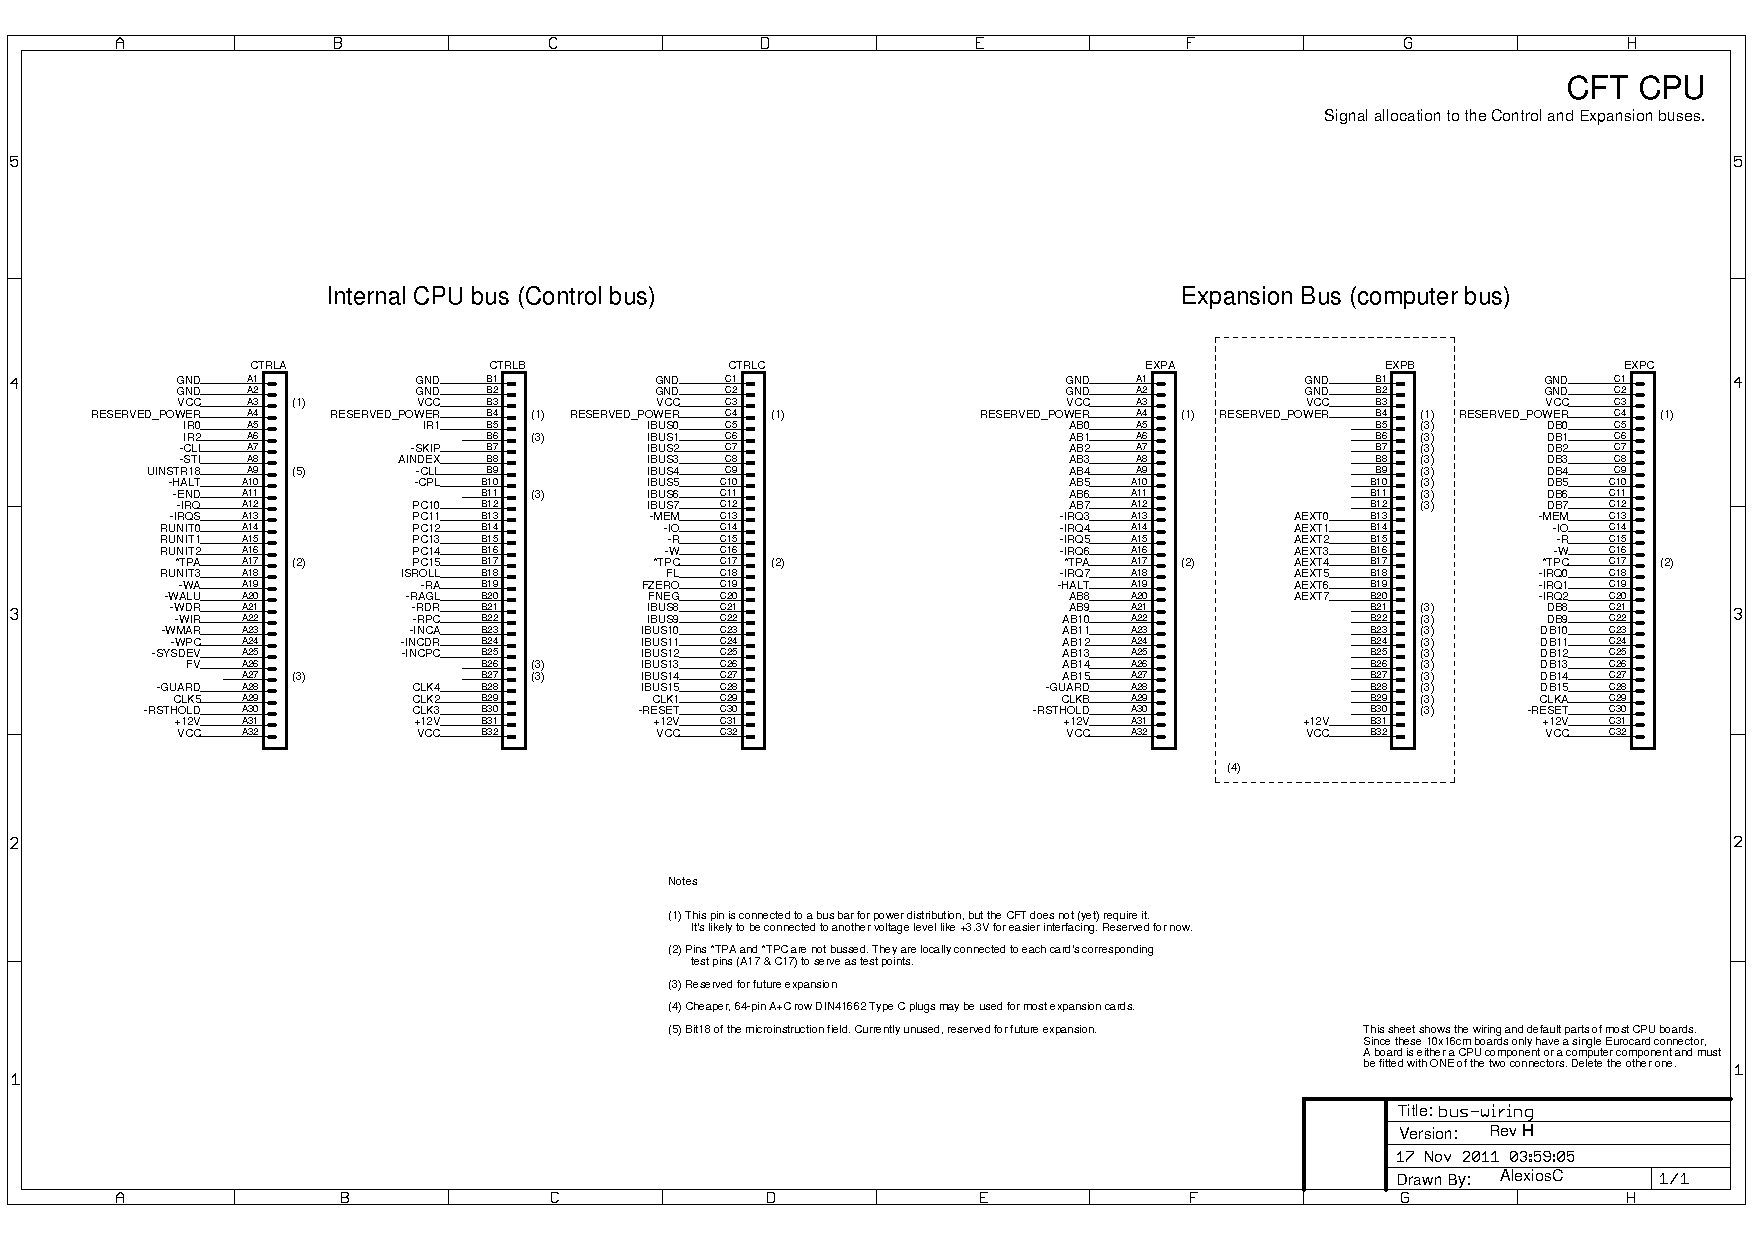
\includegraphics[width=0.95\textheight,angle=90]{figs/bus-wiring.pdf}\\
%% \caption{\label{fig-schematic-bus-wiring}Schematic drawing of the bus wiring.}
%% \end{figure*}


%%  LocalWords:  documentclass CFT Alexios PDP autoindexing Von LSI Chouchoulas
%%  LocalWords:  Neumann microprograms microprogram microinstructions Bauform
%%  LocalWords:  et cetera kiloword KWord kilowords KWords Autoindex rp GND CLC
%%  LocalWords:  SUBRET JSR TRAPRET ISRRET ISR autoindex th FC FFF tl RSTIN tri
%%  LocalWords:  FFFF pagerel vlgrey linewidth fillstyle fillcolor de GPULSE
%%  LocalWords:  addr FFFE IOT LIA JMP bitwise ORred asm bitfield CLA DMA IRQ
%%  LocalWords:  CLL RBL RBR RNL RNR NOP linearc SNA SZA SSL SNN SNZ
%%  LocalWords:  SCL CLI STI SNP lll RET RTT SBL SBR SNL SNR TTY
%%  LocalWords:  disjuncted conjuncted ANDed
